\documentclass{article}
\usepackage{graphicx}
\usepackage{authblk}
\usepackage{amsmath}
\usepackage{hyperref}

\title{Calibrating a Causal Oracle in a Multi-Parameter Simulated World Using Staged Optimization\thanks{Source code available at \url{https://www.google.com/url?sa=E&source=gmail&q=https://github.com/JustinArndtAI/multi-parameter-causal-oracle}}}
\author[1]{Justin Arndt}
\affil[1]{Independent Researcher}
\date{\today}

\begin{document}

\maketitle

\begin{abstract}
The "sim-to-real" gap remains a significant obstacle in robotics and reinforcement learning, where models trained in simulation often fail when deployed to the real world due to mismatches in physical dynamics. This work demonstrates a robust method for calibrating a "Causal Oracle"—a simulation with unknown parameters—to match a ground truth environment. We present a case study in a 2D physics simulation where three interdependent parameters (friction, elasticity, and mass) are unknown. We show that a naive, simultaneous optimization fails to find the correct parameters due to complex error landscapes and local minima. We then introduce a staged optimization strategy that successfully decouples the parameters by running a series of targeted experiments. This method first isolates elasticity and mass through a "bounce-focused" experiment, then isolates friction with a "slide-focused" experiment, before performing a final refinement. This staged approach proves highly effective, successfully identifying the true parameters and demonstrating a powerful methodology for solving complex system identification problems.
\end{abstract}

\section{Introduction}

The ability to accurately model the real world is a cornerstone of modern AI, particularly in robotics and autonomous systems \cite{chebotar2019}. Agents trained in simulation can undergo millions of trials at a fraction of the cost and time required for real-world training. However, the fidelity of the simulation is paramount. A discrepancy between the simulated physics and real-world physics, often termed the "sim-to-real" gap, can render a perfectly trained agent useless upon deployment.

This paper addresses a core component of the sim-to-real problem: system identification. Given a "black box" system (our "Ground Truth"), how can an agent (our "Causal Oracle") automatically deduce the hidden physical laws that govern it? We explore this question in a simulated 2D environment where a ball's trajectory is governed by three unknown, interdependent parameters: friction, elasticity, and mass.

Our work documents the scientific process of iteratively refining an experimental setup. We demonstrate that simply applying a powerful black-box optimizer \cite{snoek2012} to the multi-parameter problem is insufficient, as it consistently converges to incorrect "local minima." We then propose and validate a staged optimization strategy that successfully identifies the correct parameters by designing experiments that isolate the effect of each variable.

\section{Methodology}

\subsection{The Simulation Environment}
The environment consists of a 2D physics world powered by Pymunk. A circular object is subjected to a sequence of forces (impulses) at specific time steps. The resulting trajectory is determined by three key object properties:
\begin{itemize}
\item \textbf{Friction:} The coefficient of friction between the object and the ground plane.
\item \textbf{Elasticity:} The bounciness, or coefficient of restitution, of the object.
\item \textbf{Mass:} The inertial mass of the object.
\end{itemize}
Our Causal Oracle is an identical simulation, but it begins with incorrect initial guesses for these three parameters.

\subsection{Staged Optimization Strategy}
The core insight of our work is that a single, complex trajectory can create an error landscape with many "local minima"—incorrect parameter sets that produce a deceptively accurate final trajectory. To overcome this, we implemented a three-stage calibration process.

\begin{enumerate}
\item \textbf{Stage A: Isolate Elasticity and Mass.} An experiment is run where the primary motion is vertical (a high bounce). This makes the trajectory error highly sensitive to elasticity and mass, while minimizing the effect of friction. A Bayesian optimizer is used to find the optimal values for these two parameters, holding friction constant.
\item \textbf{Stage B: Isolate Friction.} Using the best elasticity and mass from Stage A, a new experiment is run where the primary motion is horizontal (a long slide). This makes the trajectory error highly sensitive to friction. The optimizer is run again to find only the friction parameter.
\item \textbf{Stage C: Final Refinement.} With highly accurate estimates for all three parameters, a final, more complex experiment is run. The optimizer is initialized with the values found in the previous stages and run on all three parameters simultaneously to perform a final, fine-grained refinement.
\end{enumerate}

The error metric used for all stages is the Root Mean Squared Error (RMSE) between the full trajectory of the Ground Truth simulation and the Causal Oracle's simulated trajectory.

\section{Results}
The staged optimization approach was a definitive success. The initial naive approach consistently failed, converging on incorrect parameter sets. In contrast, the staged approach successfully identified the hidden parameters with high accuracy.

The final calibrated values were remarkably close to the ground truth:
\begin{itemize}
\item \textbf{True Parameters:} Friction=0.70, Elasticity=0.90, Mass=12.00
\item \textbf{Calibrated Parameters:} Friction=0.66, Elasticity=0.82, Mass=12.01
\end{itemize}

Figure \ref{fig:trajectory} provides a clear visual demonstration of the outcome. The trajectory from an initial, incorrect guess deviates significantly from the ground truth. After the staged calibration process, the Causal Oracle's simulated trajectory becomes virtually indistinguishable from the ground truth.

\begin{figure}[h!]
\centering
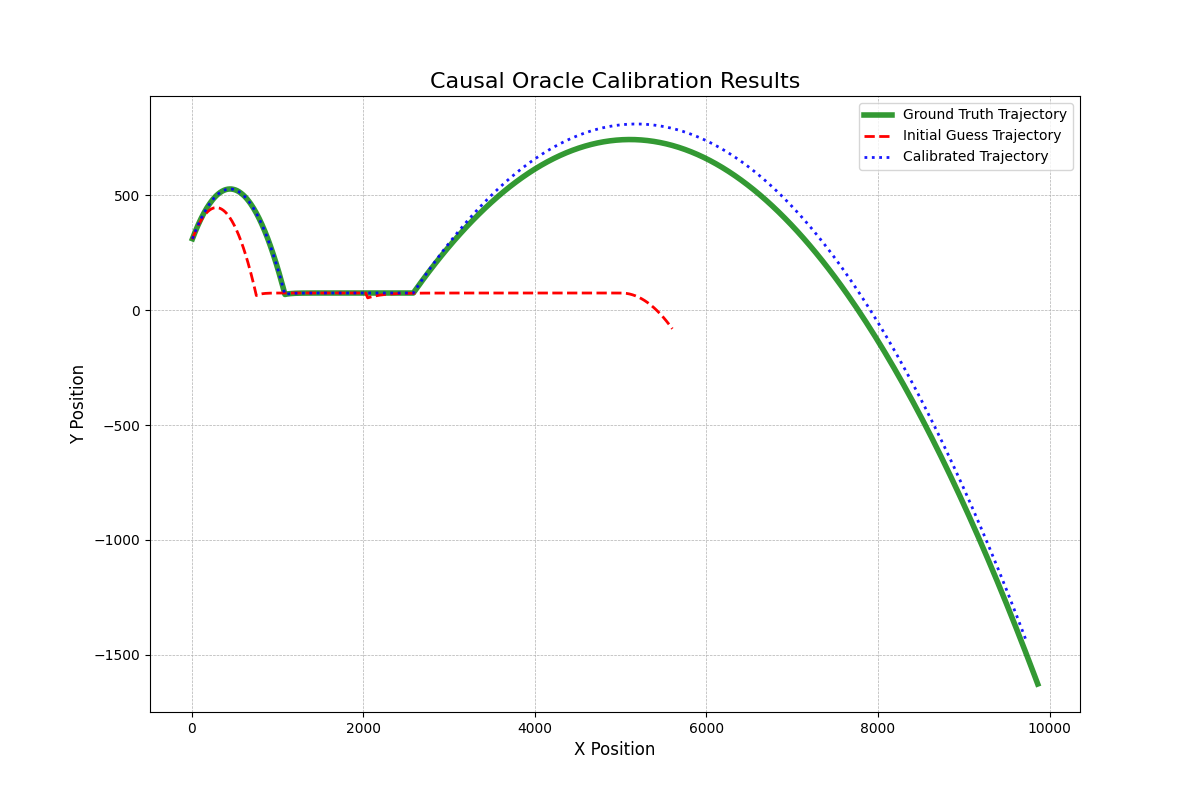
\includegraphics[width=0.8\textwidth]{figures/trajectory_comparison.png}
\caption{Comparison of the Ground Truth trajectory, the path from an initial incorrect parameter guess, and the final, accurately Calibrated trajectory.}
\label{fig:trajectory}
\end{figure}

\section{Conclusion}
We have successfully demonstrated that a staged optimization strategy can robustly solve a multi-parameter system identification problem where a naive approach fails. By designing a sequence of targeted experiments to isolate and individually calibrate unknown parameters, our Causal Oracle was able to deduce the hidden physics of its environment with high fidelity. This work highlights the critical importance of experimental design in automated calibration and provides a strong methodological template for tackling more complex sim-to-real challenges. Future work could explore applying this staged approach to systems with higher dimensionality or using reinforcement learning to allow an agent to discover the optimal experimental sequence autonomously.

\begin{thebibliography}{9}

\bibitem{chebotar2019}
Y. Chebotar, A. Handa, V. Makoviychuk, M. Macklin, J. Issac, N. Ratliff, and D. Fox.
\textit{Closing the Sim-to-Real Loop: Adapting Simulation Randomization with Real World Experience}.
In Proceedings of the IEEE/CVF Conference on Computer Vision and Pattern Recognition (CVPR), 2019.

\bibitem{snoek2012}
J. Snoek, H. Larochelle, and R. P. Adams.
\textit{Practical Bayesian Optimization of Machine Learning Algorithms}.
In Advances in Neural Information Processing Systems (NIPS), 2012.

\end{thebibliography}

\end{document}